\chapter{Concentración y dilución}\label{ch:g10:concentration-and-dilution}

Una bolsa de suero cuelga sobre la cama de un paciente. Su etiqueta
dice ``cloruro de sodio 0.9 \%'': sal en agua, nada más. Pero esa cifra,
0.9, no es un detalle. Con demasiado poca sal, las células de la sangre
del paciente se hincharían de agua; con demasiada, se arrugarían. Una
disolución no se describe solo por sus ingredientes, sino por la
cantidad de \omterm{def:g6:solutions-and-solubility:solute}{soluto} que contiene cada volumen de ella, su concentración.
Este capítulo mide concentraciones, prepara disoluciones de
concentración exacta y las diluye.

\begin{recall}
Una disolución está formada por un \omterm{def:g6:solutions-and-solubility:solute}{disolvente} y uno o varios \omterm{def:g6:solutions-and-solubility:solute}{solutos}
disueltos; la \omterm{def:g6:solutions-and-solubility:solubility}{solubilidad} es la mayor masa de \omterm{def:g6:solutions-and-solubility:solute}{soluto} que puede \omterm{def:g2:mixing-and-dissolving:dissolve}{disolver}
una cantidad dada de \omterm{def:g6:solutions-and-solubility:solute}{disolvente} (\cref{ch:g6:solutions-and-solubility}).
La cantidad de una especie es $n = m/M$, en \omterm{def:g10:the-mole:amount}{moles} (\cref{ch:g10:the-mole}).
\end{recall}

\begin{omfigure}
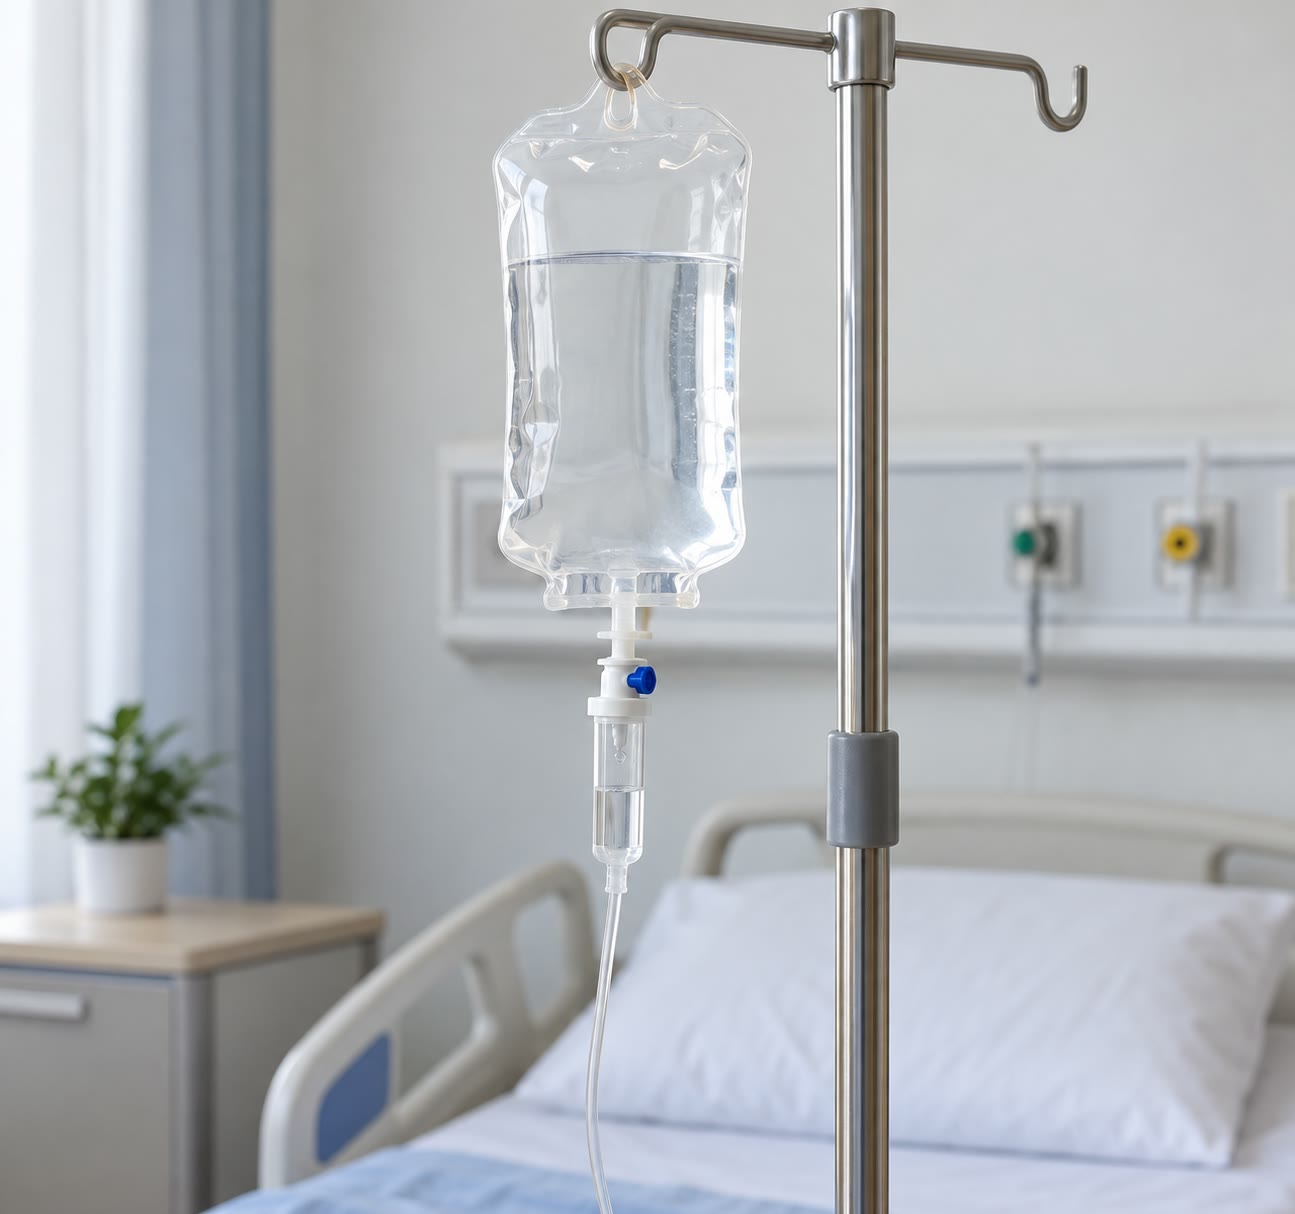
\includegraphics[width=0.42\linewidth]{images/book1/ai/g10-drip-bag.jpg}

{\small Una bolsa de suero salino: la concentración tiene que ser la
correcta.}
\end{omfigure}

\section{La concentración en masa}

\begin{definition}[Concentración en masa]\label{def:g10:concentration-and-dilution:mass-concentration}
La \emph{concentración en masa}\index{concentracion en masa@concentración en masa} $C_m$ de
un \omterm{def:g6:solutions-and-solubility:solute}{soluto} en una disolución es la masa de \omterm{def:g6:solutions-and-solubility:solute}{soluto} disuelto por volumen de
disolución:
\[
  C_m = \frac{m_{\text{soluto}}}{V_{\text{disolución}}},
\]
en gramos por litro (\si{g/L}).
\end{definition}

\begin{example}[Agua con azúcar]\label{ex:g10:concentration-and-dilution:sugar}
Se \omterm{def:g2:mixing-and-dissolving:dissolve}{disuelven} \qty{20}{g} de azúcar en agua y se completa la disolución
hasta \qty{0.50}{L}. Su \omterm{def:g10:concentration-and-dilution:mass-concentration}{concentración en masa} de azúcar es
$C_m = \qty{20}{g} / \qty{0.50}{L} = \qty{40}{g/L}$. Cualquier parte de
ella tiene la misma concentración: un vaso de \qty{0.20}{L} contiene
$\qty{40}{g/L} \times \qty{0.20}{L} = \qty{8.0}{g}$ de azúcar.
\end{example}


\begin{remark}[El volumen es el de la disolución]\label{rem:g10:concentration-and-dilution:volume}
El volumen de $C_m$ es el de toda la disolución, no el del agua que se
ha vertido: \omterm{def:g2:mixing-and-dissolving:dissolve}{disolver} un \omterm{def:g6:solutions-and-solubility:solute}{soluto} cambia un poco el volumen. Por eso una
disolución se \emph{completa} siempre hasta un volumen final conocido,
en un matraz marcado para ello.
\end{remark}

\begin{remark}[La concentración no es la solubilidad]\label{rem:g10:concentration-and-dilution:not-solubility}
% ledger: sol:NaCl, saline:NaCl
La \omterm{def:g6:solutions-and-solubility:solubility}{solubilidad} de un \omterm{def:g6:solutions-and-solubility:solute}{soluto} es la concentración \emph{máxima} que puede
alcanzar; una disolución puede tener cualquier concentración, desde cero
hasta ese valor. El cloruro de sodio se \omterm{def:g2:mixing-and-dissolving:dissolve}{disuelve} hasta unos
\qty{360}{g} por kilogramo de agua a \qty{25}{\celsius}; la bolsa de
suero solo contiene \qty{9}{g} por litro, muy lejos de la saturación.
\end{remark}

\begin{remark}[Los porcentajes de las etiquetas]\label{rem:g10:concentration-and-dilution:percent}
% ledger: saline:NaCl
En las etiquetas de medicamentos y alimentos, ``0.9 \%'' para un sólido
disuelto en agua suele significar \qty{0.9}{g} de \omterm{def:g6:solutions-and-solubility:solute}{soluto} por
\qty{100}{mL} de disolución. En gramos por litro es diez veces más: la
bolsa de suero contiene \qty{9.0}{g/L} de cloruro de sodio.
\end{remark}

\section{La concentración molar}

\begin{definition}[Concentración molar]\label{def:g10:concentration-and-dilution:molar-concentration}
La \emph{concentración molar}\index{concentracion molar@concentración molar} $c$ de un
\omterm{def:g6:solutions-and-solubility:solute}{soluto} en una disolución es la cantidad de \omterm{def:g6:solutions-and-solubility:solute}{soluto} disuelto por volumen
de disolución:
\[
  c = \frac{n_{\text{soluto}}}{V_{\text{disolución}}},
\]
en \omterm{def:g10:the-mole:amount}{moles} por litro (\si{mol/L}).
\end{definition}

\begin{proposition}[De una concentración a la otra]\label{prop:g10:concentration-and-dilution:link}
Para un \omterm{def:g6:solutions-and-solubility:solute}{soluto} de \omterm{def:g10:the-mole:molar-mass}{masa molar} $M$,
\[
  C_m = c \times M .
\]
\end{proposition}

\begin{proof}
$C_m = m / V = (n \times M) / V = (n / V) \times M = c \times M$.
\end{proof}

\begin{example}[La bolsa de suero, en moles]\label{ex:g10:concentration-and-dilution:drip}
% ledger: saline:NaCl, saline:Na, aw:Na, aw:Cl
La bolsa de suero contiene \qty{9.0}{g/L} de cloruro de sodio, de \omterm{def:g10:the-mole:molar-mass}{masa
molar} \qty{58.5}{g/mol}. Su \omterm{def:g10:concentration-and-dilution:molar-concentration}{concentración molar} es
\[
  c = \frac{C_m}{M} = \frac{\qty{9.0}{g/L}}{\qty{58.5}{g/mol}}
    = \qty{0.154}{mol/L}.
\]
La etiqueta del fabricante da la misma cifra al revés: 154 milésimas de
\omterm{def:g10:the-mole:amount}{mol} de \omterm{def:g9:ions:ion}{iones} sodio por litro.
\end{example}

\begin{remark}[Los iones en disolución]\label{rem:g10:concentration-and-dilution:ions}
El cloruro de sodio se \omterm{def:g2:mixing-and-dissolving:dissolve}{disuelve} en forma de \omterm{def:g9:ions:ion}{iones} separados \ce{Na+} y
\ce{Cl-} (\cref{ch:g9:ions}): una disolución de cloruro de sodio de
\qty{0.154}{mol/L} contiene \qty{0.154}{mol/L} de \omterm{def:g9:ions:ion}{iones} sodio y
\qty{0.154}{mol/L} de \omterm{def:g9:ions:ion}{iones} cloruro. Cómo se separa un sólido iónico en
el agua es el tema de un capítulo posterior.
\end{remark}

\begin{omfigure}
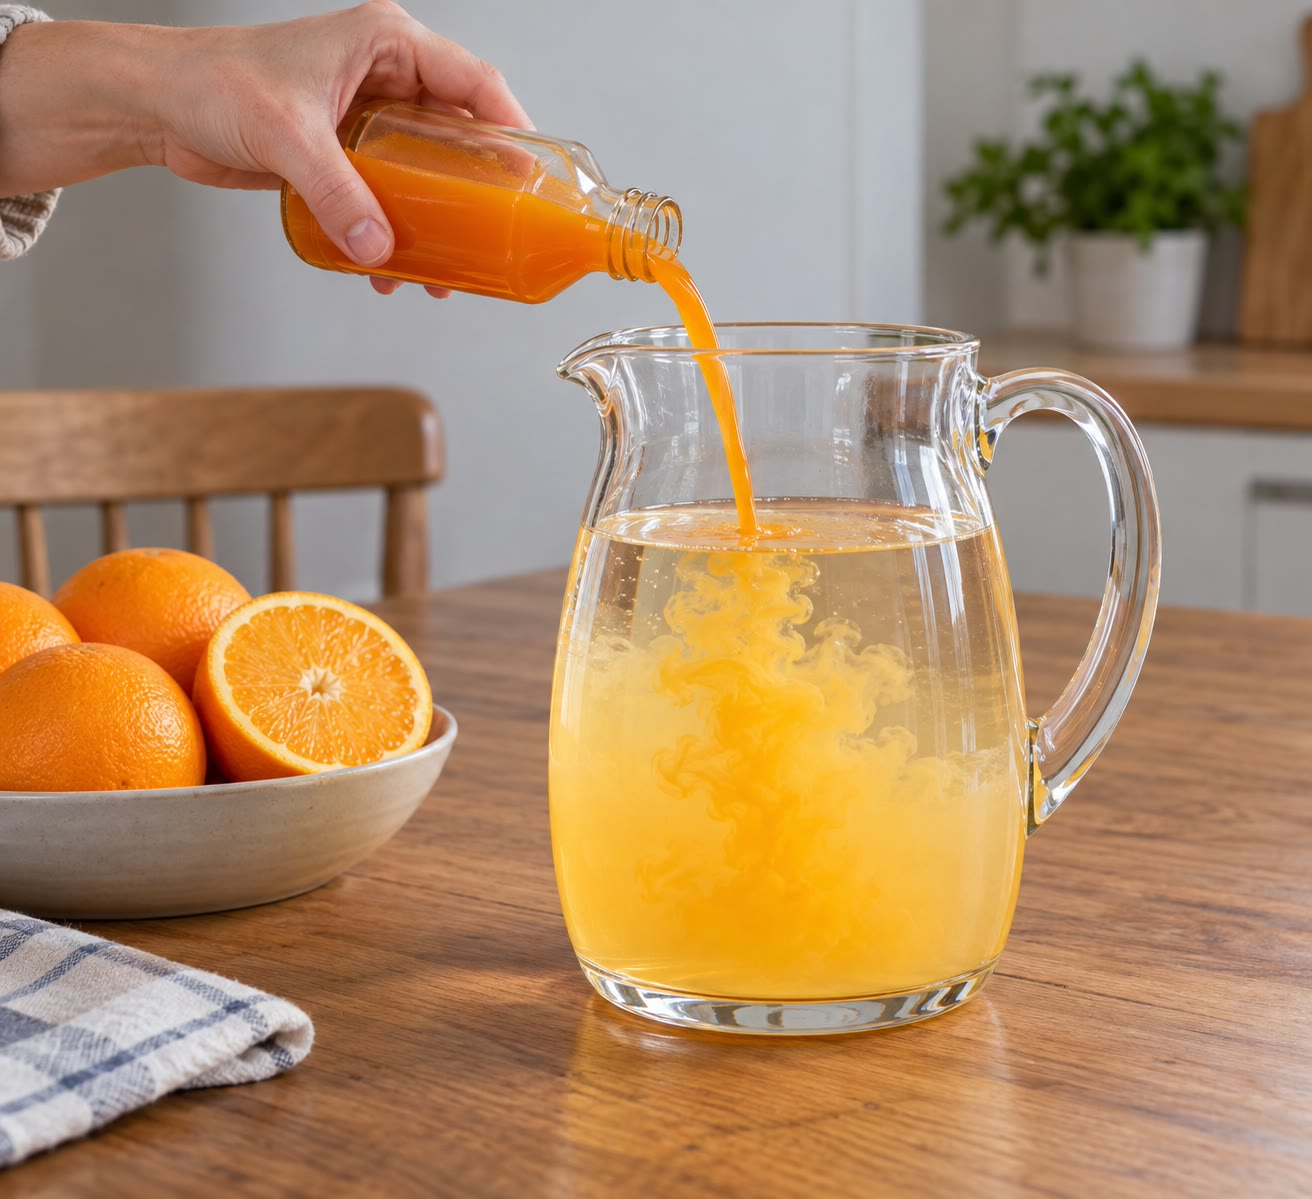
\includegraphics[width=0.45\linewidth]{images/book1/ai/g10-squash-jug.jpg}

{\small El concentrado de fruta de la botella se diluye con agua en una
jarra: la bebida contiene la misma cantidad de jarabe, en un volumen
mayor.}
\end{omfigure}

\section{Preparar una disolución por disolución de un sólido}

\begin{method}[Preparar una disolución disolviendo un sólido]\label{met:g10:concentration-and-dilution:dissolving}
Para preparar un volumen $V$ de disolución de \omterm{def:g10:concentration-and-dilution:molar-concentration}{concentración molar} $c$:
\begin{enumerate}
  \item Calcular la cantidad necesaria, $n = c \times V$, y la masa que
        hay que pesar, $m = n \times M$.
  \item Pesar esa masa de sólido en un recipiente pequeño sobre una
        balanza.
  \item Verter el sólido con un embudo en un matraz aforado de volumen
        $V$; enjuagar el recipiente y el embudo con agua destilada sobre
        el matraz, para no perder nada de sólido.
  \item Añadir agua destilada hasta más o menos la mitad del matraz y
        agitar con movimientos circulares hasta que se haya disuelto todo
        el sólido.
  \item Añadir agua destilada hasta el enrase, las últimas gotas con un
        cuentagotas; tapar el matraz e invertirlo varias veces para
        homogeneizar.
\end{enumerate}
\end{method}

\begin{omfigure}
\begin{tikzpicture}[font=\small, scale=1.05]
  % 1. weigh
  \pic[transform shape] at (0,0) {balance};
  \fill[black!8, draw=black!55] (-0.45,0.8) -- (0.45,0.8) -- (0.38,0.98)
    -- (-0.38,0.98) -- cycle;
  \fill[white, draw=black!40] (-0.25,0.98) .. controls (-0.1,1.15) and
    (0.1,1.15) .. (0.25,0.98) -- cycle;
  \node[align=center, anchor=north] at (0,-0.2) {1. pesar\\ el sólido};
  % 2. transfer through a funnel
  \pic[transform shape] at (3.2,0) {volflask={0.08}{omWater}};
  \pic[transform shape] at (3.2,3.0) {funnel};
  \draw[omProp, thick, -{Stealth}] (2.4,5.0) -- (2.85,4.65);
  \node[align=center, anchor=north] at (3.2,-0.2) {2. trasvasar,\\ enjuagar};
  % 3. half full, swirl
  \pic[transform shape] at (6.4,0) {volflask={0.45}{omWater}};
  \draw[omProp, thick, -{Stealth}] (5.55,0.5) arc[start angle=200,
    end angle=340, x radius=0.9, y radius=0.3];
  \node[align=center, anchor=north] at (6.4,-0.2) {3. a media altura:\\ agitar para disolver};
  % 4. to the mark
  \pic[transform shape] at (9.6,0) {volflask={1}{omWater}};
  \fill[black!45] (9.43,3.6) rectangle (9.77,3.85);
  \draw[omDef, thick, <-] (9.82,2.9) -- (10.6,3.3) node[right] {enrase};
  \node[align=center, anchor=north] at (9.6,-0.2) {4. llenar hasta el enrase,\\
    tapar, homogeneizar};
\end{tikzpicture}

{\small Preparación de una disolución \omterm{def:g2:mixing-and-dissolving:dissolve}{disolviendo} un sólido: pesar,
trasvasar, \omterm{def:g2:mixing-and-dissolving:dissolve}{disolver} y completar hasta el enrase del matraz aforado.}
\end{omfigure}

\begin{inthelab}[Llenar hasta el enrase]
El enrase de un matraz aforado es un anillo grabado alrededor de su
cuello. El agua de un tubo de vidrio estrecho no termina plana: su
superficie se curva hacia abajo en el centro y forma un menisco. El
matraz está lleno cuando la parte \emph{inferior} del menisco toca el
enrase, mirando con el ojo a la altura de la marca, de modo que la parte
delantera y la trasera del anillo se vean como una sola línea. Mirado
desde arriba o desde abajo, el nivel puede parecer correcto sin serlo.
\end{inthelab}

\begin{omfigure}
\begin{tikzpicture}[font=\small]
  \newcommand{\neck}[2]{% x, meniscus bottom height
    \fill[omWater] (#1-0.5,0) -- (#1-0.5,{#2+0.25}) .. controls
      (#1-0.25,#2) and (#1+0.25,#2) .. (#1+0.5,{#2+0.25}) -- (#1+0.5,0) -- cycle;
    \draw[black!60, line width=0.8pt] (#1-0.5,0) -- (#1-0.5,3);
    \draw[black!60, line width=0.8pt] (#1+0.5,0) -- (#1+0.5,3);
    \draw[omDef, line width=0.9pt] (#1-0.5,1.5) -- (#1+0.5,1.5);
    \draw[black!50] (#1-0.5,{#2+0.25}) .. controls (#1-0.25,#2) and
      (#1+0.25,#2) .. (#1+0.5,{#2+0.25});}
  \newcommand{\eye}[2]{% x, y: an eye looking to the right
    \draw[black!70] (#1-0.25,#2) .. controls (#1-0.1,#2+0.18) and
      (#1+0.1,#2+0.18) .. (#1+0.2,#2) .. controls (#1+0.1,#2-0.18) and
      (#1-0.1,#2-0.18) .. (#1-0.25,#2);
    \fill[black!70] (#1+0.05,#2) circle (0.06);}
  % right
  \neck{1.5}{1.5}
  \eye{-0.4}{1.5}
  \draw[dashed, black!50] (-0.1,1.5) -- (2.4,1.5);
  \node[align=center] at (1.5,-0.55) {correcto: ojo a la altura,\\ fondo en el enrase};
  % too high
  \neck{6}{1.85}
  \eye{4.1}{1.85}
  \draw[dashed, black!50] (4.4,1.85) -- (6.9,1.85);
  \node[align=center] at (6,-0.55) {demasiada agua:\\ menisco por encima};
  % too low
  \neck{10.5}{0.85}
  \eye{8.6}{0.85}
  \draw[dashed, black!50] (8.9,0.85) -- (11.4,0.85);
  \node[align=center] at (10.5,-0.55) {demasiado poca agua:\\ menisco por debajo};
\end{tikzpicture}

{\small El cuello de un matraz aforado, ampliado y visto con el ojo a la
altura del menisco. La línea azul es el enrase. Solo el matraz de la
izquierda está bien lleno.}
\end{omfigure}

\section{Diluir}

\begin{definition}[Dilución, disolución madre, factor de dilución]\label{def:g10:concentration-and-dilution:dilution}
Una \emph{dilución}\index{dilucion@dilución} disminuye la concentración de una
disolución añadiendo \omterm{def:g6:solutions-and-solubility:solute}{disolvente}. La disolución concentrada de partida es
la \emph{disolución madre}\index{disolucion madre@disolución madre}. El \emph{factor de
dilución}\index{factor de dilucion@factor de dilución} $F$ es el cociente entre la
concentración de la disolución madre y la de la disolución diluida:
\[
  F = \frac{c_{\text{madre}}}{c_{\text{diluida}}} .
\]
\end{definition}

\begin{proposition}[La cantidad de soluto se conserva]\label{prop:g10:concentration-and-dilution:kept}
Durante una \omterm{def:g10:concentration-and-dilution:dilution}{dilución}, la cantidad de \omterm{def:g6:solutions-and-solubility:solute}{soluto} no cambia: si un volumen
$V_0$ de \omterm{def:g10:concentration-and-dilution:dilution}{disolución madre} de concentración $c_0$ se completa hasta un
volumen $V_1$, la disolución diluida tiene la concentración $c_1$ dada
por
\[
  c_0 \times V_0 = c_1 \times V_1,
  \qquad\text{así que}\qquad
  F = \frac{c_0}{c_1} = \frac{V_1}{V_0} .
\]
Lo mismo vale para las \omterm{def:g10:concentration-and-dilution:mass-concentration}{concentraciones en masa}.
\end{proposition}

\begin{proof}
Solo se añade \omterm{def:g6:solutions-and-solubility:solute}{disolvente}: el \omterm{def:g6:solutions-and-solubility:solute}{soluto} tomado con el volumen $V_0$, una
cantidad $c_0 V_0$, está todo en el volumen final $V_1$, donde forma la
cantidad $c_1 V_1$.
\end{proof}


\begin{method}[Preparar una disolución por dilución]\label{met:g10:concentration-and-dilution:diluting}
Para preparar un volumen $V_1$ de disolución de concentración $c_1$ a
partir de una \omterm{def:g10:concentration-and-dilution:dilution}{disolución madre} de concentración $c_0$:
\begin{enumerate}
  \item Calcular el volumen de \omterm{def:g10:concentration-and-dilution:dilution}{disolución madre} que hay que tomar,
        $V_0 = c_1 V_1 / c_0$ (es decir, $V_1 / F$).
  \item Verter un poco de \omterm{def:g10:concentration-and-dilution:dilution}{disolución madre} en un vaso de precipitados
        limpio (no pipetear nunca directamente del frasco) y tomar
        exactamente $V_0$ con una pipeta aforada, llenada hasta su
        enrase.
  \item Vaciar la pipeta en un matraz aforado de volumen $V_1$.
  \item Añadir agua destilada hasta el enrase, tapar y homogeneizar.
\end{enumerate}
\end{method}

\begin{example}[Una dilución por diez]\label{ex:g10:concentration-and-dilution:tenfold}
Una \omterm{def:g10:concentration-and-dilution:dilution}{disolución madre} de sulfato de cobre tiene $c_0 = \qty{0.10}{mol/L}$;
hacen falta \qty{100.0}{mL} a $c_1 = \qty{0.010}{mol/L}$. El \omterm{def:g10:concentration-and-dilution:dilution}{factor de
dilución} es $F = 0.10 / 0.010 = 10$, así que $V_0 = \qty{100.0}{mL} / 10 =
\qty{10.0}{mL}$: una pipeta de \qty{10.0}{mL} y un matraz de
\qty{100.0}{mL}.
\end{example}

\begin{omfigure}
\begin{tikzpicture}[font=\small, scale=0.85]
  % 1. take the stock with a pipette
  \pic[transform shape] at (0,0) {beaker={0.6}{cyan!70!blue!55}};
  \pic[transform shape] at (0,0.2) {pipette={1}{cyan!70!blue!55}};
  \node[align=center, anchor=north] at (0,-0.2) {1. pipetear $V_0$\\ de disolución madre};
  \draw[omProp, very thick, -{Stealth}] (1.3,2.6) -- (2.6,2.6);
  % 2. empty it into the flask
  \pic[transform shape] at (4,0) {volflask={0.22}{cyan!70!blue!55}};
  \pic[transform shape] at (4,2.6) {pipette={0.12}{cyan!70!blue!55}};
  \node[align=center, anchor=north] at (4,-0.2) {2. vaciarla en\\ el matraz};
  \draw[omProp, very thick, -{Stealth}] (5.3,2.6) -- (6.6,2.6);
  % 3. water to the mark
  \pic[transform shape] at (8,0) {volflask={1}{cyan!70!blue!14}};
  \draw[omDef, thick, <-] (8.2,2.9) -- (9.1,3.4) node[right] {enrase};
  \node[align=center, anchor=north] at (8,-0.2) {3. agua hasta el enrase:\\
    volumen $V_1$};
\end{tikzpicture}

{\small \omterm{def:g10:concentration-and-dilution:dilution}{Dilución}: un volumen $V_0$ de \omterm{def:g10:concentration-and-dilution:dilution}{disolución madre}, medido con una
pipeta, se completa hasta $V_1$ en un matraz aforado. El color se
atenúa según el \omterm{def:g10:concentration-and-dilution:dilution}{factor de dilución} $V_1 / V_0$.}
\end{omfigure}

\section{Una escala de patrones}

\begin{definition}[Disolución patrón, escala de patrones]\label{def:g10:concentration-and-dilution:standard}
Una \emph{disolución patrón}\index{disolucion patron@disolución patrón} es una disolución
cuya concentración se conoce con precisión. Una \emph{escala de
patrones}\index{escala de patrones} es una serie de disoluciones patrón
del mismo \omterm{def:g6:solutions-and-solubility:solute}{soluto}, de concentraciones crecientes, que se suelen preparar
diluyendo una misma \omterm{def:g10:concentration-and-dilution:dilution}{disolución madre}; al comparar con ella una
disolución desconocida se obtiene una estimación de su concentración.
\end{definition}

\begin{example}[Una escala azul]\label{ex:g10:concentration-and-dilution:scale}
A partir de una \omterm{def:g10:concentration-and-dilution:dilution}{disolución madre} de sulfato de cobre de
\qty{0.20}{mol/L}, se preparan seis patrones de 0.02, 0.04, 0.06, 0.08,
0.10 y \qty{0.12}{mol/L}, cada uno en tubos idénticos llenos hasta la
misma altura. Una disolución de concentración desconocida, en el mismo
tipo de tubo, se ve más oscura que el tubo de \qty{0.06}{mol/L} y más
clara que el de \qty{0.08}{mol/L}: su concentración está entre las dos,
alrededor de \qty{0.07}{mol/L}.
\end{example}

\begin{omfigure}
\begin{tikzpicture}[font=\small]
  \foreach \i/\c/\p in {0/0.02/8, 1/0.04/16, 2/0.06/24, 3/0.08/32,
                        4/0.10/40, 5/0.12/48} {
    \pic at (1.2*\i,0) {testtube={0.75}{cyan!70!blue!\p}};
    \node[anchor=north] at (1.2*\i,-0.15) {\c};
  }
  \pic at (8.4,0) {testtube={0.75}{cyan!70!blue!28}};
  \node[anchor=north] at (8.4,-0.15) {?};
  \draw[black!40] (7.55,-0.6) -- (7.55,3.2);
  \node[anchor=north] at (3,-0.7) {concentración (\si{mol/L})};
  \node[anchor=north] at (8.4,-0.7) {desconocida};
\end{tikzpicture}

{\small Una \omterm{def:g10:concentration-and-dilution:standard}{escala de patrones} de disoluciones de sulfato de cobre y una
disolución desconocida. La desconocida está entre el tercer y el cuarto
tubo.}
\end{omfigure}

\begin{safety}{\ghs[0.82cm]{GHS05}\ghs[0.82cm]{GHS07}\ghs[0.82cm]{GHS09}}
% ledger: ghs:CuSO4
Disoluciones de sulfato de cobre: nocivas en caso de ingestión,
irritantes para la piel, dañinas para los ojos, muy tóxicas para los
organismos acuáticos. Gafas y guantes; las disoluciones usadas se
recogen para tratarlas y nunca se tiran por el fregadero.
\end{safety}

\begin{remark}[Los límites del ojo]\label{rem:g10:concentration-and-dilution:eye}
El ojo solo puede decir ``entre estos dos tubos''. Para medir con más
finura una concentración a partir del color de una disolución, los
químicos miden cuánta luz absorbe; un capítulo posterior hace
exactamente eso.
\end{remark}

\section{Ejercicios}

\begin{exercise}[$\star$]\label{exo:g10:concentration-and-dilution:1}
Se \omterm{def:g2:mixing-and-dissolving:dissolve}{disuelven} \qty{5.0}{g} de azúcar para obtener \qty{250}{mL} de
disolución. Calcula la \omterm{def:g10:concentration-and-dilution:mass-concentration}{concentración en masa} de azúcar en gramos por
litro.
\end{exercise}

\begin{exercise}[$\star$]\label{exo:g10:concentration-and-dilution:2}
Una disolución de \qty{200}{mL} contiene \qty{0.050}{mol} de glucosa.
Calcula su \omterm{def:g10:concentration-and-dilution:molar-concentration}{concentración molar}.
\end{exercise}

\begin{exercise}[$\star$]\label{exo:g10:concentration-and-dilution:3}
¿Qué masa de sulfato de cobre anhidro \ce{CuSO4} hay que pesar para
preparar \qty{100.0}{mL} de disolución de \qty{0.10}{mol/L}?
\end{exercise}

\begin{exercise}[$\star$]\label{exo:g10:concentration-and-dilution:4}
Una \omterm{def:g10:concentration-and-dilution:dilution}{disolución madre} de \qty{1.0}{mol/L} se diluye hasta
\qty{0.050}{mol/L}. ¿Cuál es el \omterm{def:g10:concentration-and-dilution:dilution}{factor de dilución}? ¿Qué volumen de
\omterm{def:g10:concentration-and-dilution:dilution}{disolución madre} hace falta para preparar \qty{100.0}{mL} de disolución
diluida?
\end{exercise}

\begin{exercise}[$\star$]\label{exo:g10:concentration-and-dilution:5}
Una disolución de cloruro de sodio tiene una \omterm{def:g10:concentration-and-dilution:molar-concentration}{concentración molar} de
\qty{0.10}{mol/L}. ¿Cuál es su \omterm{def:g10:concentration-and-dilution:mass-concentration}{concentración en masa}?
\end{exercise}

\begin{exercise}[$\star\star$]\label{exo:g10:concentration-and-dilution:6}
¿Qué volumen de una \omterm{def:g10:concentration-and-dilution:dilution}{disolución madre} de \qty{0.50}{mol/L} hay que tomar
para preparar \qty{250.0}{mL} de disolución de \qty{0.020}{mol/L}?
Nombra los dos instrumentos de vidrio que se usan.
\end{exercise}

\begin{exercise}[$\star\star$]\label{exo:g10:concentration-and-dilution:7}
¿Por qué una disolución de concentración exacta se prepara en un matraz
aforado y no en un vaso de precipitados graduado? ¿Por qué un volumen de
\omterm{def:g10:concentration-and-dilution:dilution}{disolución madre} se mide con una pipeta aforada y no con una probeta?
\end{exercise}

\begin{exercise}[$\star\star$]\label{exo:g10:concentration-and-dilution:8}
Mira la \omterm{def:g10:concentration-and-dilution:standard}{escala de patrones} de sulfato de cobre. Una segunda disolución
desconocida es más clara que el tubo de \qty{0.04}{mol/L} pero más
oscura que el de \qty{0.02}{mol/L}. Estima su concentración. ¿Cómo se
podría cambiar la escala para estimarla con más precisión?
\end{exercise}

\begin{exercise}[$\star\star$]\label{exo:g10:concentration-and-dilution:9}
Una disolución de glucosa para perfusión contiene \qty{50}{g/L} de
glucosa \ce{C6H12O6}. Calcula su \omterm{def:g10:concentration-and-dilution:molar-concentration}{concentración molar}.
\end{exercise}

\begin{exercise}[$\star\star$]\label{exo:g10:concentration-and-dilution:10}
Se prepara un jarabe \omterm{def:g2:mixing-and-dissolving:dissolve}{disolviendo} \qty{342}{g} de sacarosa
\ce{C12H22O11} hasta obtener \qty{1.00}{L} de disolución. Calcula su
\omterm{def:g10:concentration-and-dilution:molar-concentration}{concentración molar}. Después se diluye diez veces. ¿Qué masa de
sacarosa contiene una cucharada de \qty{20}{mL} del jarabe diluido?
\end{exercise}

\begin{exercise}[$\star\star$]\label{exo:g10:concentration-and-dilution:11}
Una disolución tiene una \omterm{def:g10:concentration-and-dilution:mass-concentration}{concentración en masa} de \qty{12}{g/L}. ¿Cuál
es su concentración (a) después de añadir agua hasta duplicar su
volumen; (b) después de \omterm{def:g3:separating-mixtures:evaporate}{evaporar} la mitad de su agua, quedando todo el
\omterm{def:g6:solutions-and-solubility:solute}{soluto} disuelto?
\end{exercise}

\begin{exercise}[$\star\star\star$]\label{exo:g10:concentration-and-dilution:12}
Una disolución de \qty{0.10}{mol/L} se diluye diez veces, el resultado
se vuelve a diluir diez veces, y otra vez más.
\begin{enumerate}
  \item ¿Cuál es la concentración final?
  \item ¿Por qué se hace en tres pasos y no en una sola \omterm{def:g10:concentration-and-dilution:dilution}{dilución} por 1000
        (piensa en los volúmenes del material de vidrio necesario)?
\end{enumerate}
\end{exercise}

\begin{exercise}[$\star\star\star$]\label{exo:g10:concentration-and-dilution:13}
Se \omterm{def:g2:mixing-and-dissolving:dissolve}{disuelven} \qty{11.1}{g} de cloruro de calcio \ce{CaCl2} para obtener
\qty{500.0}{mL} de disolución. En el agua, el sólido se separa en \omterm{def:g9:ions:ion}{iones}
calcio \ce{Ca^2+} e \omterm{def:g9:ions:ion}{iones} cloruro \ce{Cl-}.
\begin{enumerate}
  \item Calcula la \omterm{def:g10:concentration-and-dilution:molar-concentration}{concentración molar} de cloruro de calcio disuelto.
  \item Deduce las \omterm{def:g10:concentration-and-dilution:molar-concentration}{concentraciones molares} de los \omterm{def:g9:ions:ion}{iones} calcio y de los
        \omterm{def:g9:ions:ion}{iones} cloruro de la disolución.
\end{enumerate}
\end{exercise}

\begin{exercise}[$\star\star\star$]\label{exo:g10:concentration-and-dilution:14}
Un matraz aforado de \qty{100.0}{mL} tiene un cuello de diámetro
interior \qty{1.2}{cm}. Un alumno lo llena con la parte inferior del
menisco \qty{2}{mm} por encima del enrase.
\begin{enumerate}
  \item ¿Qué volumen de agua de más ha añadido (volumen de un cilindro:
        $\pi r^2 h$)?
  \item ¿En qué porcentaje es demasiado baja la concentración de la
        disolución?
\end{enumerate}
\end{exercise}

\begin{exercise}[$\star\star\star$]\label{exo:g10:concentration-and-dilution:15}
Se \omterm{def:g2:mixing-and-dissolving:mix}{mezclan} \qty{100}{mL} de disolución de cloruro de sodio de
\qty{0.20}{mol/L} con \qty{300}{mL} de disolución de cloruro de sodio de
\qty{0.10}{mol/L}. Suponiendo que los volúmenes se suman, calcula la
concentración de la \omterm{def:g6:pure-substances-and-mixtures:mixture}{mezcla}. ¿Es la media de las dos concentraciones?
Explícalo.
\end{exercise}

\section{Problema: La bolsa de suero}

\begin{problem}[{Problema de fin de semana --- ¿cuánta disolución
concentrada de sal va en una bolsa de suero ``0.9 \%''?}]
\label{pb:g10:concentration-and-dilution:1}
% ledger: saline:NaCl, saline:Na, sol:NaCl, aw:Na, aw:Cl, const:NA
El laboratorio de la farmacia de un hospital tiene una disolución
concentrada estéril de cloruro de sodio que contiene \qty{200}{g/L} (en
su etiqueta: ``20 \%''). Tiene que preparar bolsas de \qty{500}{mL} de
la disolución ``0.9 \%'' que se usa en los goteros, diluyendo la
disolución concentrada con agua estéril.

\medskip
\noindent\textbf{Parte I --- Qué significa 0.9 \%.}
\begin{enumerate}
  \item La etiqueta ``0.9 \%'' significa \qty{0.9}{g} de sal por
        \qty{100}{mL} de disolución. Da la \omterm{def:g10:concentration-and-dilution:mass-concentration}{concentración en masa} en
        \si{g/L}.
  \item Exprésala también en miligramos por mililitro.
  \item ¿Qué masa de cloruro de sodio contiene una bolsa de
        \qty{500}{mL}?
  \item El cloruro de sodio se \omterm{def:g2:mixing-and-dissolving:dissolve}{disuelve} hasta unos \qty{360}{g} por
        kilogramo de agua. ¿Está la disolución de la bolsa lejos de la
        saturación?
  \item Un paciente recibe \qty{1.0}{L} de esta disolución en un día.
        ¿Qué masa de sal es eso?
\end{enumerate}

\medskip
\noindent\textbf{Parte II --- En \omterm{def:g10:the-mole:amount}{moles}.}
\begin{enumerate}[resume]
  \item Calcula la \omterm{def:g10:the-mole:molar-mass}{masa molar} del cloruro de sodio.
  \item Calcula la \omterm{def:g10:concentration-and-dilution:molar-concentration}{concentración molar} de la disolución de la bolsa.
  \item ¿Qué cantidad de cloruro de sodio contiene una bolsa?
  \item ¿Cuáles son las \omterm{def:g10:concentration-and-dilution:molar-concentration}{concentraciones molares} de los \omterm{def:g9:ions:ion}{iones} sodio y de
        los \omterm{def:g9:ions:ion}{iones} cloruro de la bolsa?
  \item ¿Cuántos \omterm{def:g9:ions:ion}{iones} sodio contiene una bolsa?
\end{enumerate}

\medskip
\noindent\textbf{Parte III --- A partir de la disolución concentrada.}
\begin{enumerate}[resume]
  \item Calcula el \omterm{def:g10:concentration-and-dilution:dilution}{factor de dilución} entre la disolución concentrada y
        la disolución de la bolsa.
  \item ¿Qué masa de cloruro de sodio tiene que venir de la disolución
        concentrada para una bolsa? Deduce el volumen de disolución
        concentrada que hay que tomar.
  \item Comprueba este volumen con el \omterm{def:g10:concentration-and-dilution:dilution}{factor de dilución}.
  \item Calcula la \omterm{def:g10:concentration-and-dilution:molar-concentration}{concentración molar} de la disolución concentrada y
        comprueba que $c_0 V_0 = c_1 V_1$.
  \item ¿Qué volumen de agua estéril, más o menos, se añade entonces
        (suponiendo que los volúmenes se suman)?
\end{enumerate}

\medskip
\noindent\textbf{Parte IV --- El material de vidrio y la exactitud.}
\begin{enumerate}[resume]
  \item No existe ninguna pipeta aforada de este volumen. ¿Qué
        instrumento de vidrio, graduado en décimas de mililitro, podría
        medirlo?
  \item ¿En qué recipiente habría que completar el volumen final para
        que sea exacto?
  \item Si se tomaran \qty{23.0}{mL} en lugar del volumen correcto, ¿qué
        \omterm{def:g10:concentration-and-dilution:mass-concentration}{concentración en masa} tendría la bolsa? ¿En qué porcentaje sería
        errónea?
  \item Da la respuesta final: ¿qué volumen de la disolución concentrada
        va en una bolsa de \qty{500}{mL}?
\end{enumerate}
\end{problem}
